% unit: u39
% sources: sources/071-final-course-review.txt, sources/230-final-course-review.txt, sources/231-mit18-06scf11-finalrevsum-pdf-download-file.txt, sources/020-final-exam-problem-solving.txt
\section{Final course review}\label{sec:u39}

The final exam covers the whole course, and its best questions connect the parts: a question about solvability turns into a question about $A\T A$; a Markov matrix is solved by noticing that it is singular. The way to review is to work old final-exam problems, and that is what this section does after a one-page summary of the tools they use. Even the ``easy'' material from the first third of the course does real work here.

\subsection{The toolkit}

\begin{enumerate}[(1)]
\item \emph{Rank and solvability} (Sections~\ref{sec:u09}--\ref{sec:u11}). For $m\times n$ $A$ of rank $r$: $A\vb{x}=\vb{b}$ is solvable for every $\vb{b}$ iff $r=m$; solutions are unique (when they exist) iff $r=n$, i.e.\ $\Nul{A}=\{\vb{0}\}$. The dimensions are $r$, $n-r$, $r$, $m-r$ for $\Col{A\T},\Nul{A},\Col{A},\Nul{A\T}$.
\item \emph{The matrix $A\T A$} (Sections~\ref{sec:u18} and~\ref{sec:u36}). It is square, symmetric and positive semidefinite, and $\Nul{A\T A}=\Nul{A}$; so it is invertible (indeed positive definite) iff $r=n$.
\item \emph{Projections and least squares} (Sections~\ref{sec:u17}--\ref{sec:u18}). $A\T A\hat{\vb{x}}=A\T\vb{b}$, $\vb{p}=A\hat{\vb{x}}$, $P=A(A\T A)^{-1}A\T$; the error $\vb{e}=\vb{b}-\vb{p}$ lies in $\Nul{A\T}$. For a line, $P=\vb{a}\vb{a}\T/\vb{a}\T\vb{a}$.
\item \emph{Eigenvalue shortcuts} (Sections~\ref{sec:u23}--\ref{sec:u26}). Sum $=\tr A$, product $=\det A$; singular $\Rightarrow\lambda=0$; Markov $\Rightarrow\lambda=1$; $A+cI$ has $\lambda+c$; triangular matrices show their eigenvalues on the diagonal; $A=X\Lambda X^{-1}$ builds a matrix from given eigenvalues and eigenvectors.
\item \emph{Special matrices} (Section~\ref{sec:u37}). Symmetric, skew-symmetric, orthogonal, projection, permutation, Markov, positive definite: each has a signature in its eigenvalues and eigenvectors.
\end{enumerate}

\subsection{Solved problems from past finals}

\begin{example}[What one solvable and one unsolvable system reveal]\label{ex:u39-rank}
$A$ is $m\times n$ of rank $r$. $A\vb{x}=(1,0,0)$ has no solution, and $A\vb{x}=(0,1,0)$ has exactly one.

(a) \emph{What are $m,n,r$?} The right-hand sides have three components, so $m=3$. Some right-hand side is unreachable, so $\Col{A}\neq\R^{3}$ and $r<3$. A solution exists and is unique, so $\Nul{A}=\{\vb{0}\}$ and $r=n$; and $(0,1,0)\in\Col{A}$ gives $r\ge1$. In short: $m=3$ and $1\le r=n\le2$.

(b) \emph{An example.} Put $(0,1,0)$ in the column space and stop: $A=\begin{bmatrix}0\\1\\0\end{bmatrix}$ ($n=r=1$). Or add a column that keeps $(1,0,0)$ out: $A=\begin{bmatrix}0&0\\1&0\\0&1\end{bmatrix}$ ($n=r=2$).

(c) \emph{True or false for every such $A$:} (i) $\det A\T A=\det AA\T$; (ii) $A\T A$ is invertible; (iii) $AA\T$ is positive definite. Statement (ii) is true because $r=n$ (toolkit item 2); for the examples, $A\T A=I$. Statement (iii) is false: $AA\T$ is $3\times3$ with rank $n<3$, so it is singular. It is always positive \emph{semi}definite; for the second example $AA\T=\operatorname{diag}(0,1,1)$. Then (i) is false too: $\det A\T A\neq0$ but $\det AA\T=0$. The rule $\det(BA)=\det(AB)=\det A\det B$ needs square matrices.

(d) \emph{Prove that $A\T\vb{y}=\vb{c}$ has infinitely many solutions for every $\vb{c}$.} $A\T$ is $n\times3$ with rank $n$: full row rank, so a solution exists for every $\vb{c}$. Its nullspace $\Nul{A\T}$ has dimension $m-r=3-n\ge1$, and adding any multiple of a nonzero nullspace vector to one solution gives another.
\end{example}

\begin{example}[Columns $\vb{v}_1,\vb{v}_2,\vb{v}_3$]\label{ex:u39-columns}
The columns of $A$ are $\vb{v}_1,\vb{v}_2,\vb{v}_3$.
(a) $A\vb{x}=\vb{v}_1-\vb{v}_2+\vb{v}_3$ is solved by $\vb{x}=(1,-1,1)$: $A\vb{x}$ is the combination of columns with coefficients $x_j$, the very first idea of the course.
(b) \emph{True or false: if $\vb{v}_1-\vb{v}_2+\vb{v}_3=\vb{0}$, the solution in (a) is not unique.} True. Then $(1,-1,1)$ is in $\Nul{A}$, and adding any multiple of it to a solution gives another solution.
(c) \emph{If $\vb{v}_1,\vb{v}_2,\vb{v}_3$ are orthonormal, which combination of $\vb{v}_1$ and $\vb{v}_2$ is closest to $\vb{v}_3$?} The projection of $\vb{v}_3$ onto the plane of $\vb{v}_1,\vb{v}_2$ is $(\vb{v}_1\T\vb{v}_3)\vb{v}_1+(\vb{v}_2\T\vb{v}_3)\vb{v}_2=0\vb{v}_1+0\vb{v}_2$. Think of $\vb{v}_3$ as the $z$-axis and the plane as the $xy$-plane: the closest point is the origin.
\end{example}

\begin{example}[A singular Markov matrix]\label{ex:u39-markov}
$A=\begin{bmatrix}.2&.4&.3\\.4&.2&.3\\.4&.4&.4\end{bmatrix}$; note that column 1 $+$ column 2 $=2\times$ column 3.

\emph{Eigenvalues.} The columns are dependent, so $\lambda=0$. The columns sum to $1$, so $\lambda=1$ (the all-ones vector is an eigenvector of $A\T$). The trace is $0.8$, so the third is $\lambda=0.8-0-1=-0.2$.

\emph{Steady state from $\vb{u}_0=(0,10,0)$.} $\vb{u}_k=A^{k}\vb{u}_0=c_1(0)^{k}\vb{x}_1+c_2(1)^{k}\vb{x}_2+c_3(-0.2)^{k}\vb{x}_3$, so only $c_2\vb{x}_2$ survives as $k\to\infty$. For $\vb{x}_2$ solve $(A-I)\vb{x}=\vb{0}$: the matrix has columns $(-.8,.4,.4)$, $(.4,-.8,.4)$, $(.3,.3,-.6)$, and a lucky guess with $x_1=x_2$ works: $\vb{x}_2=(3,3,4)$, since $A(3,3,4)=(.6+1.2+1.2,\ 1.2+.6+1.2,\ 1.2+1.2+1.6)=(3,3,4)$. A Markov step preserves the total of the entries, which is $10$ at the start and $10$ in $(3,3,4)$, so $c_2=1$ and
\[
\vb{u}_\infty=(3,3,4).
\]
Figure~\ref{fig:u39-markov} shows the approach: the third entry is $4$ from the first step on, and the first two oscillate around $3$ because of the factor $(-0.2)^{k}$.
\end{example}

\begin{figure}[ht]\centering
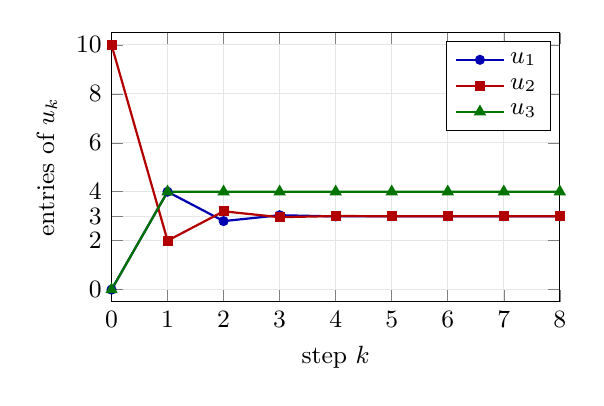
\begin{tikzpicture}
\begin{axis}[width=0.6\textwidth,height=5cm,xlabel={step $k$},ylabel={entries of $\vb{u}_k$},
  xmin=0,xmax=8,ymin=-0.5,ymax=10.5,xtick={0,1,...,8},ytick={0,2,3,4,6,8,10},grid=major,grid style={gray!20},
  legend style={font=\small,at={(0.98,0.97)},anchor=north east},font=\small]
\addplot[blue!70!black,thick,mark=*,mark size=1.4pt] coordinates {(0,0) (1,4) (2,2.8) (3,3.04) (4,2.992) (5,3.0016) (6,2.9997) (7,3.0001) (8,3)};
\addplot[red!70!black,thick,mark=square*,mark size=1.4pt] coordinates {(0,10) (1,2) (2,3.2) (3,2.96) (4,3.008) (5,2.9984) (6,3.0003) (7,2.9999) (8,3)};
\addplot[green!45!black,thick,mark=triangle*,mark size=1.8pt] coordinates {(0,0) (1,4) (2,4) (3,4) (4,4) (5,4) (6,4) (7,4) (8,4)};
\legend{$u_1$,$u_2$,$u_3$}
\end{axis}
\end{tikzpicture}
\caption{The Markov chain of Example~\ref{ex:u39-markov} from $\vb{u}_0=(0,10,0)$. The $\lambda=0$ part disappears after one step, the $\lambda=-0.2$ part shrinks by a factor $5$ and changes sign each step, and $\vb{u}_k\to(3,3,4)$.}\label{fig:u39-markov}
\end{figure}

\begin{example}[Four $2\times2$ matrices on demand]\label{ex:u39-four}
(a) \emph{The projection onto the line through $\vb{a}=(4,-3)$:} $P=\dfrac{\vb{a}\vb{a}\T}{\vb{a}\T\vb{a}}=\dfrac{1}{25}\begin{bmatrix}16&-12\\-12&9\end{bmatrix}$; as a check, $\det P=0$ and $\tr P=1$.

(b) \emph{The matrix with $\lambda=0$, $\vb{x}=(1,2)$ and $\lambda=3$, $\vb{x}=(2,1)$:}
\[
A=X\Lambda X^{-1}=\begin{bmatrix}1&2\\2&1\end{bmatrix}\begin{bmatrix}0&0\\0&3\end{bmatrix}\begin{bmatrix}-1/3&2/3\\2/3&-1/3\end{bmatrix}=\begin{bmatrix}0&6\\0&3\end{bmatrix}\begin{bmatrix}-1/3&2/3\\2/3&-1/3\end{bmatrix}=\begin{bmatrix}4&-2\\2&-1\end{bmatrix}.
\]
Check: $A(1,2)=(0,0)$ and $A(2,1)=(6,3)=3(2,1)$.

(c) \emph{A real matrix that is not $B\T B$ for any $B$:} $B\T B$ is always symmetric, so any non-symmetric matrix works, e.g.\ $\begin{bmatrix}0&0\\1&0\end{bmatrix}$. (So is any symmetric matrix with a negative eigenvalue, since $B\T B$ is semidefinite.)

(d) \emph{Orthogonal eigenvectors but not symmetric:} the skew-symmetric $\begin{bmatrix}0&1\\-1&0\end{bmatrix}$ or the rotation $\begin{bmatrix}\cos\theta&-\sin\theta\\\sin\theta&\cos\theta\end{bmatrix}$, both of which commute with their transposes; their eigenvectors $(1,\pm i)$ are complex and orthogonal.
\end{example}

\begin{example}[Least squares, given the answer]\label{ex:u39-lsq}
For $A\vb{x}=\vb{b}$ with
\[
A=\begin{bmatrix}1&0\\1&1\\1&2\end{bmatrix},\qquad \vb{b}=\begin{bmatrix}3\\4\\1\end{bmatrix},
\]
the least-squares solution is $(\hat c,\hat d)=(\tfrac{11}{3},-1)$. (Check: $A\T A=\begin{bmatrix}3&3\\3&5\end{bmatrix}$, $A\T\vb{b}=(8,6)$, and $3\cdot\tfrac{11}{3}-3=8$, $3\cdot\tfrac{11}{3}-5=6$.)

(a) \emph{The projection of $\vb{b}$ onto $\Col{A}$} is the best combination of the columns: $\vb{p}=\tfrac{11}{3}(1,1,1)-1\cdot(0,1,2)=(\tfrac{11}{3},\tfrac83,\tfrac53)$.

(b) \emph{The straight-line problem.} The rows say $C+Dt=b$ at $t=0,1,2$: fit the points $(0,3)$, $(1,4)$, $(2,1)$. The best line is $b=\tfrac{11}{3}-t$ (Figure~\ref{fig:u39-line}); the errors $\vb{e}=\vb{b}-\vb{p}=(-\tfrac23,\tfrac43,-\tfrac23)$ are perpendicular to both columns.

(c) \emph{A nonzero $\vb{b}$ whose least-squares solution is $(0,0)$.} We need $\vb{p}=\vb{0}$, i.e.\ $\vb{b}$ orthogonal to both columns, i.e.\ $\vb{b}\in\Nul{A\T}$: $\vb{b}=(1,-2,1)$ works ($1+(-2)+1=0$ and $0-2+2=0$). Notice that $\vb{e}$ in (b) is $-\tfrac23(1,-2,1)$, in the same line.
\end{example}

\begin{figure}[ht]\centering
\begin{tikzpicture}[scale=1.25,>=Stealth,font=\small]
  \draw[->] (-0.4,0) -- (3.0,0) node[right] {$t$};
  \draw[->] (0,-0.3) -- (0,4.7) node[above] {$b$};
  \foreach \y in {1,2,3,4} \draw (0.06,\y) -- (-0.06,\y) node[left] {$\y$};
  \foreach \x in {1,2} \draw (\x,0.06) -- (\x,-0.06) node[below] {$\x$};
  \draw[thick,blue!70!black] (-0.2,3.867) -- (2.7,0.967) node[right] {$b=\frac{11}{3}-t$};
  \draw[red!70!black,thick] (0,3) -- (0,3.667);
  \draw[red!70!black,thick] (1,4) -- (1,2.667);
  \draw[red!70!black,thick] (2,1) -- (2,1.667);
  \fill (0,3) circle (2pt) node[below right] {$(0,3)$};
  \fill (1,4) circle (2pt) node[above right] {$(1,4)$};
  \fill (2,1) circle (2pt) node[below right] {$(2,1)$};
  \node[red!70!black,right] at (1,3.3) {$e_2=\frac43$};
  \node[red!70!black,left] at (2,1.35) {$e_3=-\frac23$};
\end{tikzpicture}
\caption{The straight-line fit behind Example~\ref{ex:u39-lsq}. The vertical errors $e_1=-\tfrac23$, $e_2=\tfrac43$, $e_3=-\tfrac23$ are the components of $\vb{e}=\vb{b}-\vb{p}$; they sum to zero and are orthogonal to $(0,1,2)$, which is exactly $A\T\vb{e}=\vb{0}$.}\label{fig:u39-line}
\end{figure}

\begin{example}[Eigenvalues, pivots and semidefiniteness without computing]\label{ex:u39-pivots}
$A=\begin{bmatrix}1&0&1\\0&1&1\\1&1&0\end{bmatrix}$ has eigenvalues $\lambda_1=1$, $\lambda_2=2$, and its first two pivots are $1$ and $1$.

(a) \emph{The third eigenvalue and pivot.} The trace is $1+1+0=2=1+2+\lambda_3$, so $\lambda_3=-1$. Elimination without row exchanges does not change the determinant, so $d_1d_2d_3=\det A=\lambda_1\lambda_2\lambda_3=-2$, giving $d_3=-2$. (No row exchange is needed, since the first two pivots $1,1$ are nonzero, so the determinant really is the product of the three pivots.)

(b) \emph{The smallest $a_{33}$ that makes $A$ positive semidefinite.} With $a_{33}$ in the corner, elimination gives pivots $1$, $1$ and $\det A/(1\cdot1)$, where expanding the determinant gives $\det A=a_{33}-2$. A symmetric matrix factored as $LDL\T$ is semidefinite exactly when all pivots are $\ge0$, so the condition is $a_{33}\ge2$; the smallest choice is $a_{33}=2$ (the eigenvalues are then $0,1,3$).

\emph{The smallest $c$ that makes $A+cI$ positive semidefinite.} Shifting adds $c$ to each eigenvalue: $1+c$, $2+c$, $-1+c$ are all $\ge0$ exactly when $c\ge1$.
\end{example}

\begin{trap}
Positive leading determinants are a complete test for a positive definite matrix, but nonnegative leading determinants do not guarantee a semidefinite one: the diagonal matrix $\operatorname{diag}(0,-1)$ has leading determinants $0$ and $0$ but an eigenvalue $-1$. In Example~\ref{ex:u39-pivots} the argument works because the first two pivots are strictly positive, so the last pivot alone decides.
\end{trap}

\subsection{Exercises}

\begin{exercise}\label{exr:u39-halfA}
With $A$ as in Example~\ref{ex:u39-pivots}, let $\vb{u}_{k+1}=\tfrac12A\vb{u}_k$ and start from $(3,0,0)$, $(0,3,0)$ or $(0,0,3)$. Find $\lim_{k\to\infty}\vb{u}_k$.
\end{exercise}
\begin{solution}
Each column of $A$ sums to $2$, so $\tfrac12A$ is a Markov matrix. It has zero entries, so the usual guarantee of a unique steady state (for positive matrices) does not apply directly; check the eigenvalues instead. They are half of $1,2,-1$: $\tfrac12$, $1$, $-\tfrac12$. Only one has absolute value $1$, so $\vb{u}_k$ converges to a multiple of its eigenvector. Each row of $A$ also sums to $2$, so $A(1,1,1)=(2,2,2)$ and the eigenvector is $(1,1,1)$. A Markov step preserves the total $3$, so in all three cases
\[
\lim_{k\to\infty}\vb{u}_k=(1,1,1).
\]
\end{solution}

\begin{exercise}\label{exr:u39-P}
For the matrix $A$ of Example~\ref{ex:u39-lsq}, compute the projection matrix $P=A(A\T A)^{-1}A\T$ and check that $P\vb{b}=\vb{p}$ and $P(1,-2,1)=\vb{0}$.
\end{exercise}
\begin{solution}
$(A\T A)^{-1}=\frac16\begin{bmatrix}5&-3\\-3&3\end{bmatrix}$, and
\[
P=\frac16\begin{bmatrix}1&0\\1&1\\1&2\end{bmatrix}\begin{bmatrix}5&-3\\-3&3\end{bmatrix}\begin{bmatrix}1&1&1\\0&1&2\end{bmatrix}=\frac16\begin{bmatrix}5&2&-1\\2&2&2\\-1&2&5\end{bmatrix}.
\]
Then $P\vb{b}=\frac16(15+8-1,\ 6+8+2,\ -3+8+5)=\frac16(22,16,10)=(\tfrac{11}{3},\tfrac83,\tfrac53)=\vb{p}$, and $P(1,-2,1)=\frac16(5-4-1,\ 2-4+2,\ -1-4+5)=\vb{0}$.
\end{solution}

\begin{exercise}\label{exr:u39-variant}
Change Example~\ref{ex:u39-rank}: $A\vb{x}=(1,0,0)$ still has no solution, but $A\vb{x}=(0,1,0)$ now has infinitely many. What can you say about $m,n,r$? Which of the statements in (c) and (d) change?
\end{exercise}
\begin{solution}
Still $m=3$ and $1\le r<3$. Infinitely many solutions means $\Nul{A}\neq\{\vb{0}\}$, so now $r<n$ ($n$ can be anything larger than $r$). Then $A\T A$ is singular ($\Nul{A\T A}=\Nul{A}\neq\{\vb{0}\}$), so (ii) becomes false; (iii) stays false since $AA\T$ is $3\times3$ of rank $r<3$. Statement (d) fails: $A\T$ is $n\times3$ of rank $r<n$, not full row rank, so $A\T\vb{y}=\vb{c}$ is solvable only for $\vb{c}$ in the row space of $A$. Example: $A=\begin{bmatrix}0&0\\1&1\\0&0\end{bmatrix}$.
\end{solution}

\begin{exercise}\label{exr:u39-sym}
Find the symmetric $2\times2$ matrix with eigenvalue $0$ for $\vb{x}=(1,2)$ and eigenvalue $3$. Why could the matrix in Example~\ref{ex:u39-four}(b) not be symmetric?
\end{exercise}
\begin{solution}
A symmetric matrix has orthogonal eigenvectors, so $\lambda=3$ goes with $\vb{q}=(2,-1)/\sqrt5$, and $A=0\cdot(\dots)+3\vb{q}\vb{q}\T=\frac35\begin{bmatrix}4&-2\\-2&1\end{bmatrix}$. Check: $A(1,2)=\frac35(4-4,-2+2)=\vb{0}$, and $A(2,-1)=\frac35(10,-5)=3(2,-1)$. In Example~\ref{ex:u39-four}(b) the eigenvectors $(1,2)$ and $(2,1)$ have dot product $4\neq0$, and eigenvectors of a symmetric matrix for different eigenvalues are always orthogonal.
\end{solution}
